% Page Layout
\documentclass[12pt,t]{beamer}
\usepackage{etex} % Avoid an error due to a lack of registers
\usepackage[english]{babel} % Defines the language of macros as well
\usepackage{float}
\usepackage{amsmath}
\usepackage{listings}
\usepackage{geometry}
\usepackage{graphicx}
% Desired Packages
%\usepackage[pdftex]{graphicx}
\usepackage[utf8]{inputenc}
\usepackage{amsmath}
\usepackage{amssymb}
\usepackage{lastpage}
\usepackage{listings}
\usepackage{caption}
\usepackage{xy}
\usepackage{microtype}
\usepackage{lmodern, hfoldsty}
\usepackage{ellipsis}
\usepackage{tabularx}
\usepackage{beamerthemeshadow}
\usepackage{nameref}
\usepackage{hyperref}
\usepackage{subfig}
\usepackage[absolute,overlay]{textpos}
\setlength{\TPHorizModule}{\paperwidth}
\setlength{\TPHorizModule}{\paperheight}

% Further Configurations
\newcommand{\Fat}[1]{{\large \bf \textcolor{cdc_Blue}{#1}}}
\renewcommand\rmdefault{pmy}            		% Activate Myriad Font
\definecolor{Gray}{rgb}{0.5, 0.5, 0.5}  		% Define light color
\definecolor{HighlightRed}{rgb}{0.6, 0.0, 0.0}  % Define light highlighting color
\graphicspath{{images/}}
\usetheme{UniOldbg}                     		% The main thing: our theme


\title[WPMP - Energy Meteorology]{WPMP - Energy Meteorology}
\author[Jan \& Florian]{Jan Kämper \& Florian Börgel}
\date{01.06.2016}
\semester{Semester 2016}
\institute{Universität Oldenburg}

\begin{document}

\definecolor{mygreen}{rgb}{0,0.6,0}
\definecolor{mygray}{rgb}{0.5,0.5,0.5}
\definecolor{mymauve}{rgb}{0.58,0,0.82}

\lstset{ %
  backgroundcolor=\color{white},   % choose the background color; you must add \usepackage{color} or \usepackage{xcolor}
  basicstyle=\tiny,        % the size of the fonts that are used for the code
  breakatwhitespace=false,         % sets if automatic breaks should only happen at whitespace
  breaklines=true,                 % sets automatic line breaking
  captionpos=b,                    % sets the caption-position to bottom
  commentstyle=\color{mygreen},    % comment style
  deletekeywords={...},            % if you want to delete keywords from the given language
  escapeinside={\%*}{*)},          % if you want to add LaTeX within your code
  extendedchars=true,              % lets you use non-ASCII characters; for 8-bits encodings only, does not work with UTF-8
  frame=tb,	                   % adds a frame around the code
  keepspaces=true,                 % keeps spaces in text, useful for keeping indentation of code (possibly needs columns=flexible)
  keywordstyle=\color{blue},       % keyword style
  language=Octave,                 % the language of the code
  otherkeywords={*,...},           % if you want to add more keywords to the set
  numbers=left,                    % where to put the line-numbers; possible values are (none, left, right)
  numbersep=5pt,                   % how far the line-numbers are from the code
  numberstyle=\tiny\color{mygray}, % the style that is used for the line-numbers
  rulecolor=\color{black},         % if not set, the frame-color may be changed on line-breaks within not-black text (e.g. comments (green here))
  showspaces=false,                % show spaces everywhere adding particular underscores; it overrides 'showstringspaces'
  showstringspaces=false,          % underline spaces within strings only
  showtabs=false,                  % show tabs within strings adding particular underscores
  stepnumber=2,                    % the step between two line-numbers. If it's 1, each line will be numbered
  stringstyle=\color{mymauve},     % string literal style
  tabsize=2,	                   % sets default tabsize to 2 spaces
  title=\lstname                   % show the filename of files included with \lstinputlisting; also try caption instead of title
}


\frame{\titlepage}
\frame{\frametitle{Table of Contents}\tableofcontents}

\AtBeginSection[]{
	\frame{
		\frametitle{Table of Contents}
		\tableofcontents[currentsection]
	}
}

%%%%%%%%%%%% Start of content %%%%%%%%%%%% 
\section{Wind Roses}
\begin{frame}[fragile]
\frametitle{Wind Rose implementation}
\begin{lstlisting}
WindRose(fino1_d90,fino1_v90, 'AngleNorth',0,'AngleEast',90);
\end{lstlisting}
\begin{figure}
\centering
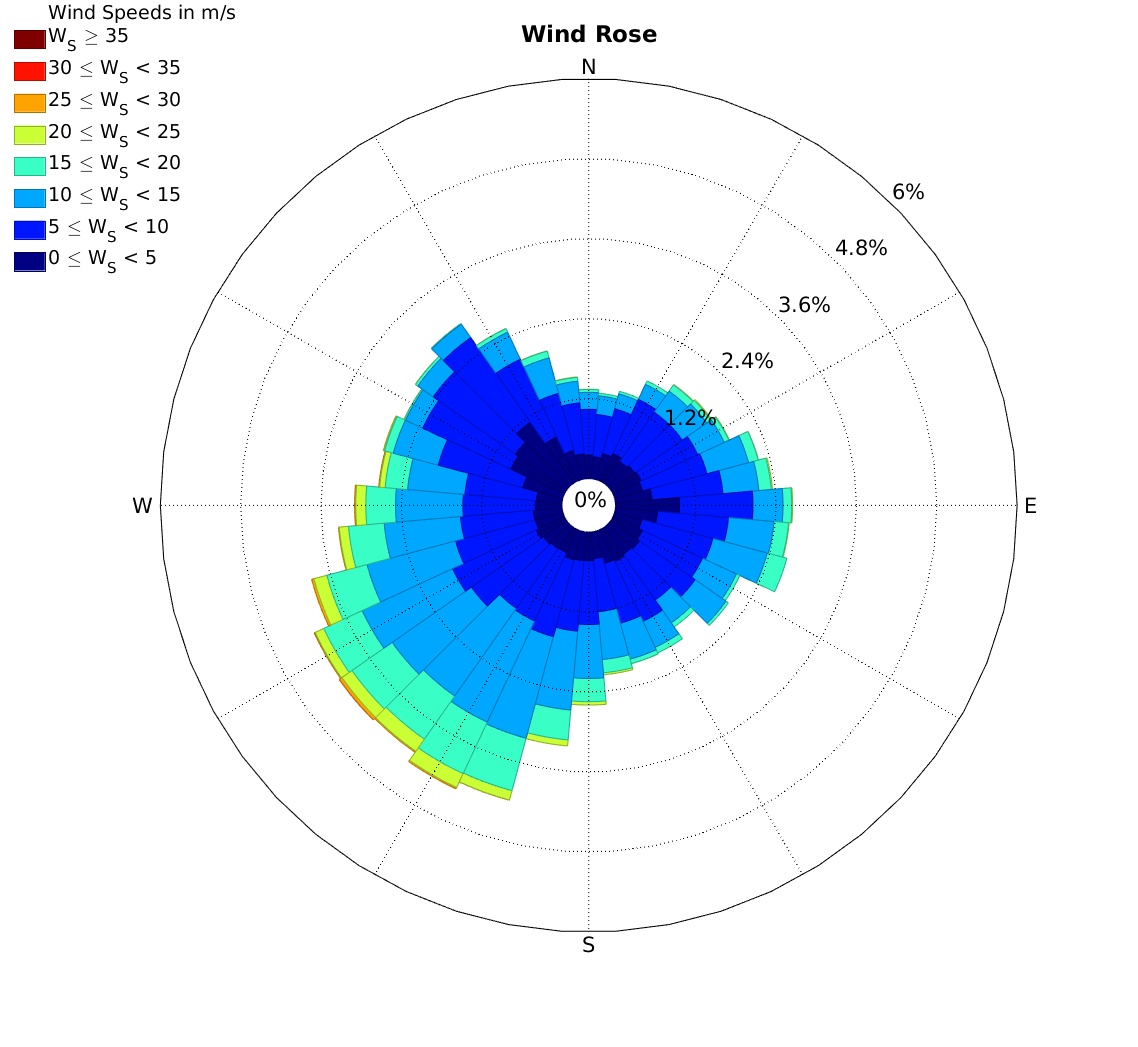
\includegraphics[width=0.45\linewidth]{../../figures/WindRose_Fino1.png}
\end{figure}

\end{frame}
\begin{frame}
	\frametitle{Wind Roses}
\begin{figure}[htbp]
	\begin{center}
		\begin{minipage}[t]{0.4\linewidth}
			\centering
			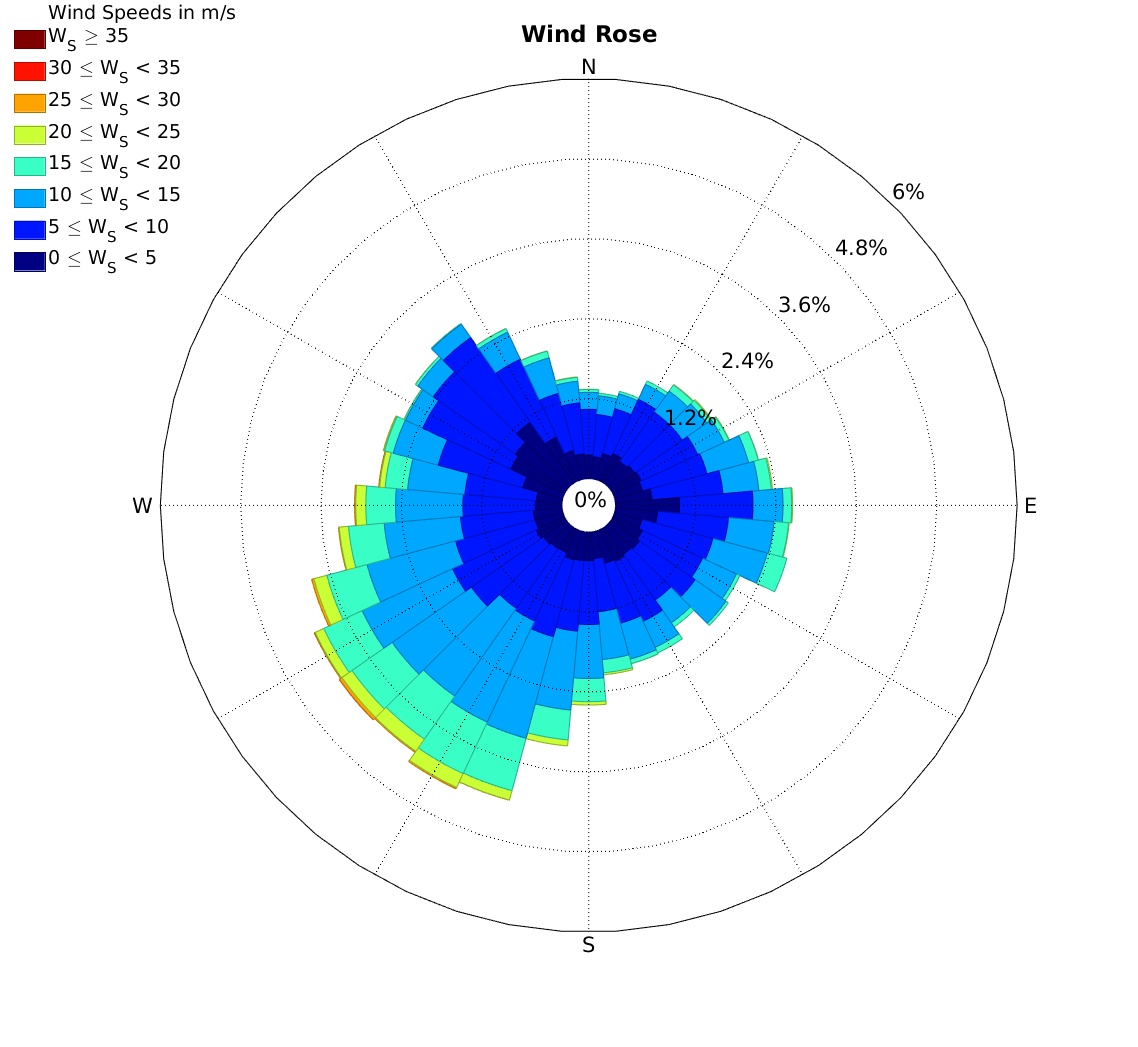
\includegraphics[width=\linewidth]{../../figures/WindRose_Fino1.png}

			\label{label 1}
		\end{minipage}
		\qquad
		\pause
		\begin{minipage}[t]{0.5\linewidth}
			\centering
			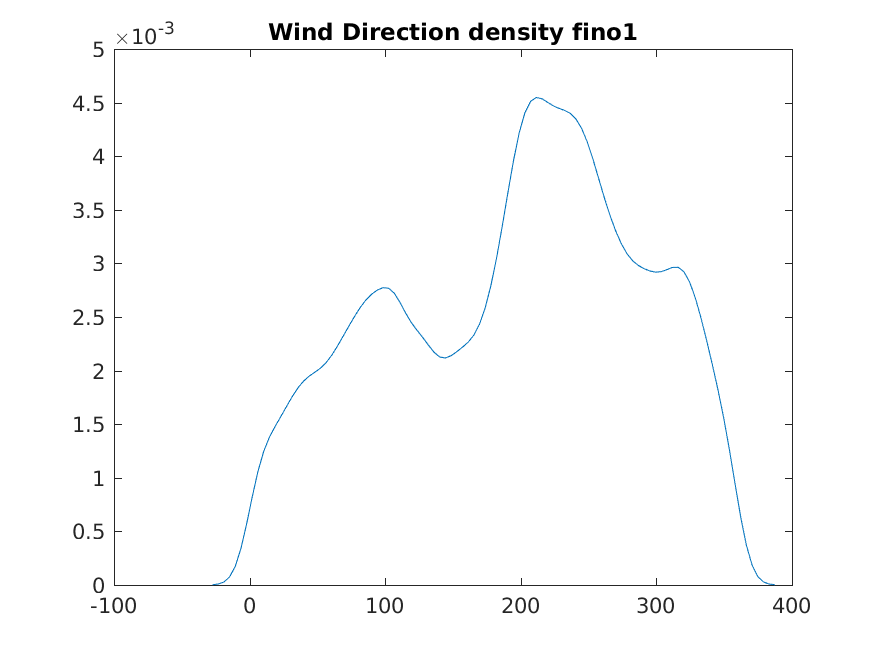
\includegraphics[width=\linewidth]{../../figures/Validation_WindRose_Fino1.png}
			\label{label 2}
		\end{minipage}
	\end{center}
\end{figure}
\end{frame}

\begin{frame}
	\frametitle{Wind Roses}
\begin{figure}[htbp]
	\begin{center}
		\begin{minipage}[t]{0.45\linewidth}
			\centering
			Fino 1
			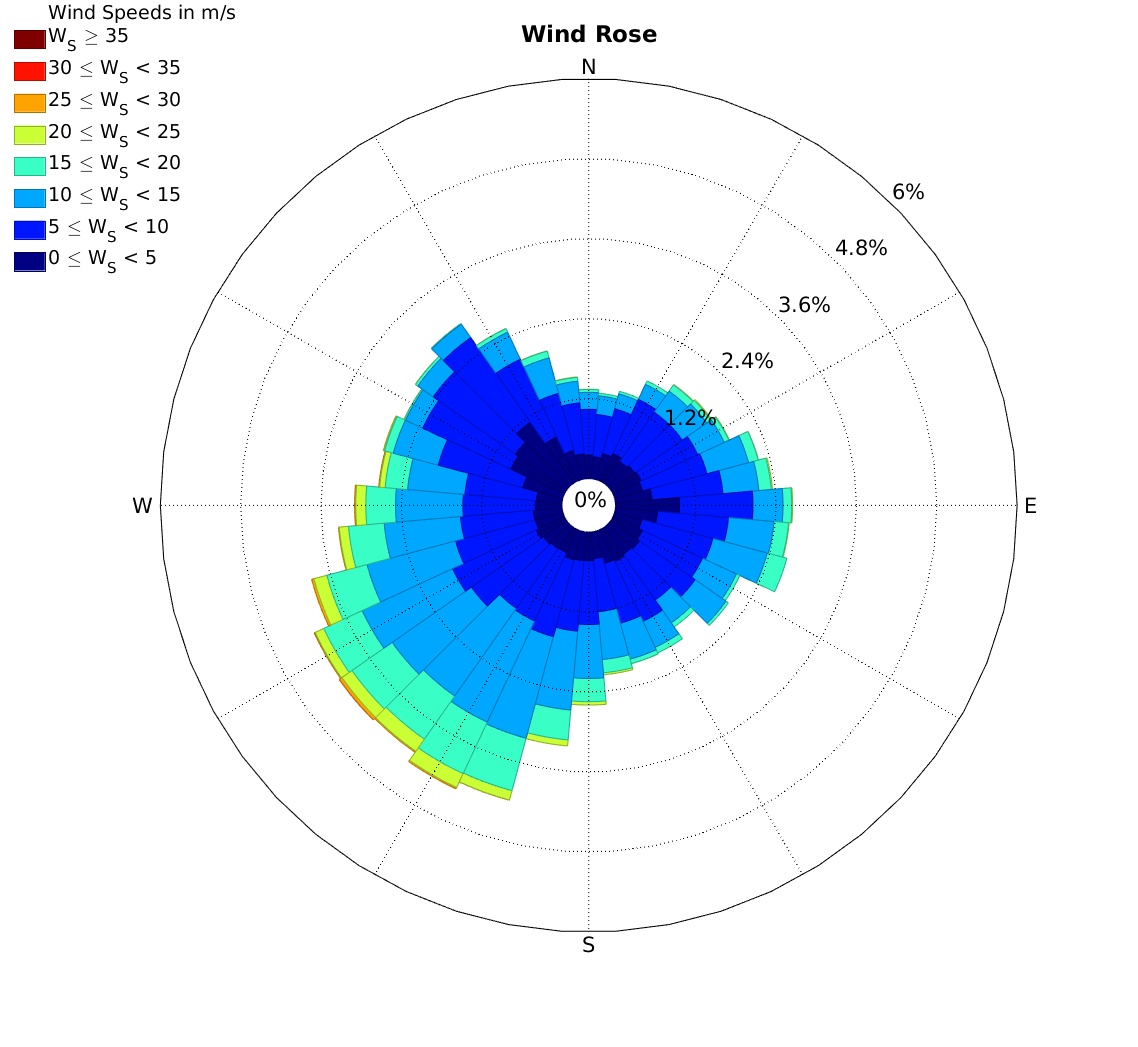
\includegraphics[width=\linewidth]{../../figures/WindRose_Fino1.png}
			\label{label 1}
		\end{minipage}
		\begin{minipage}[t]{0.45\linewidth}
			\centering
			Fino 2
			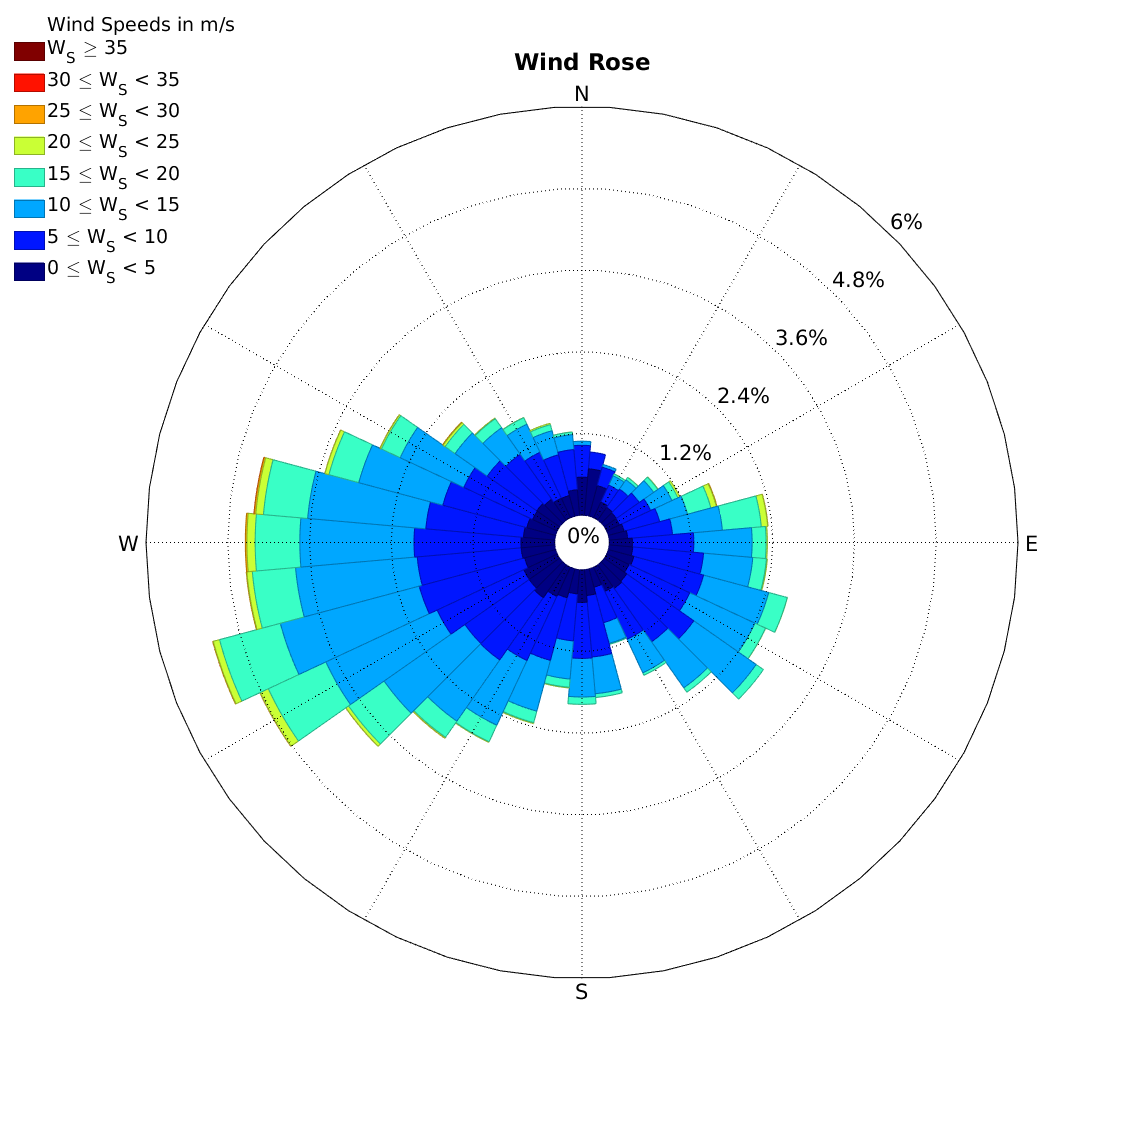
\includegraphics[width=\linewidth]{../../figures/WindRose_Fino2.png}
			\label{label 2}
		\end{minipage}
	\end{center}
\end{figure}
\end{frame}
\begin{frame}
\frametitle{Differences}
\begin{figure}[H]
\centering
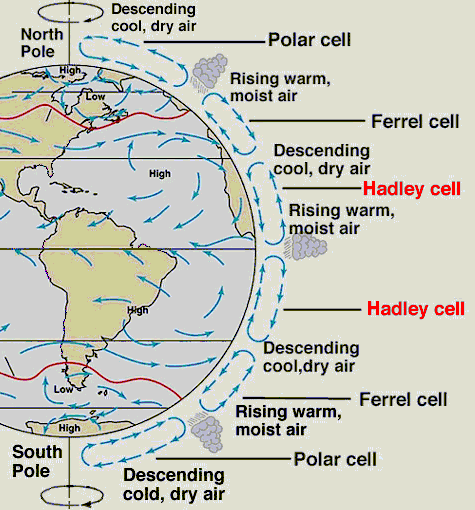
\includegraphics[width=0.5\linewidth]{../../figures/Ferrel_cell.png}
\label{fig:weatherpattern}
\end{figure}
\end{frame}


\begin{frame}
\frametitle{Differences}
\begin{figure}[H]
\centering
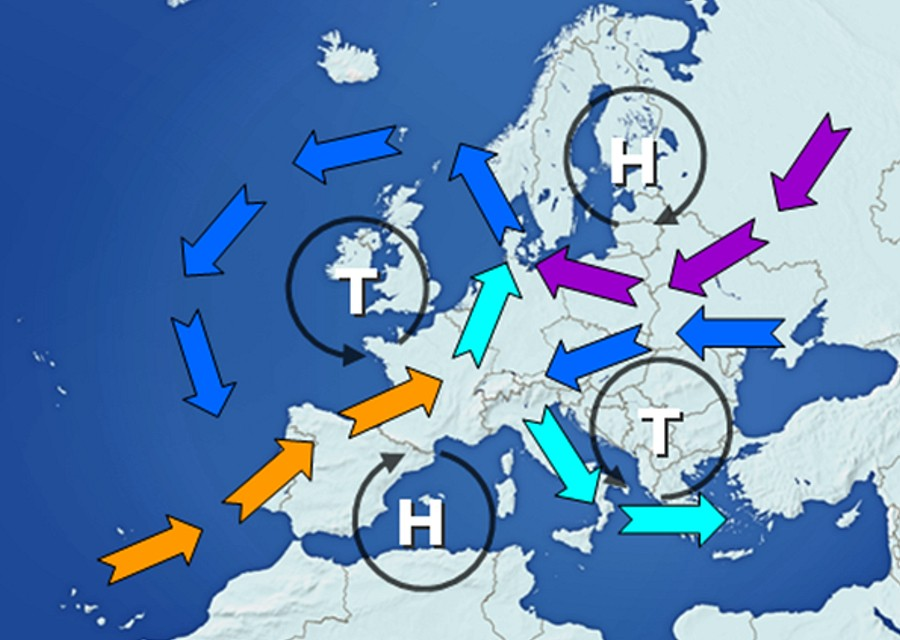
\includegraphics[width=0.7\linewidth]{../../figures/warm_air_advection.png}
\label{fig:weatherpattern}
\end{figure}
\end{frame}


\begin{frame}
\frametitle{Obstacles Fino 1}
\begin{figure}[H]
\centering
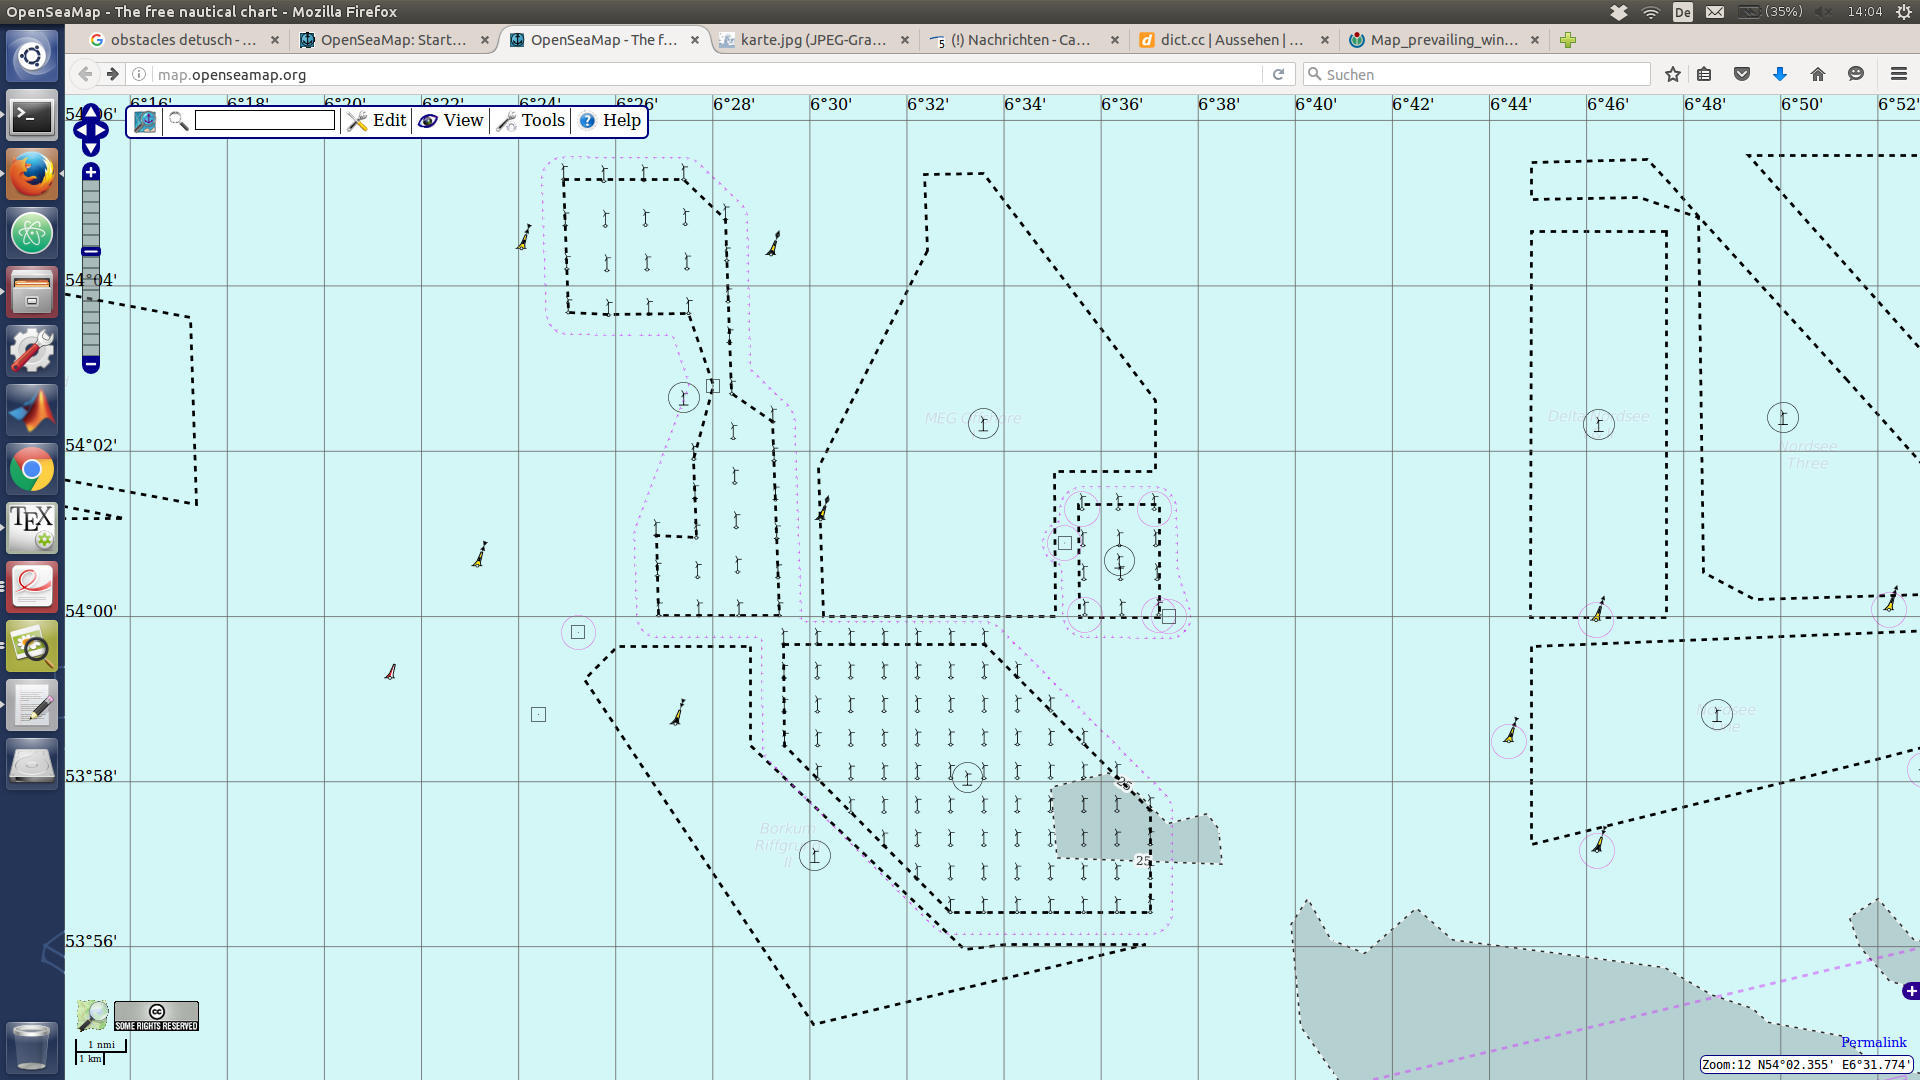
\includegraphics[width=0.8\linewidth]{../../figures/fino1.png}
\label{fig:fino1}
\end{figure} 
\end{frame}


\section{Weibull distribution}

\begin{frame}
\frametitle{Computation of Weibull parameters}
\begin{align*}
&\mu = \lambda \cdot \Gamma\left(1+\frac{1}{k}\right) \\
&\sigma^2 = \lambda^2 \cdot \left(\Gamma\left(1+\frac{2}{k}\right)-\Gamma\left(1+\frac{1}{k}\right)^2\right)
\end{align*}
By substitution:
\begin{align*}
&\sigma^2 = \left(\frac{\mu}{\Gamma(1+\frac{1}{k})}\right)^2 \cdot \left(\Gamma\left({1+\frac{2}{k}}\right)-\Gamma\left(1+\frac{1}{k}\right)^2\right)
\end{align*}
Function to solve:
\begin{align*}
&0 = \left(\frac{\mu}{\sigma}\right)^2 \cdot \left(\frac{\Gamma\left({1+\frac{2}{k}}\right)}{\Gamma\left(1+\frac{1}{k}\right)^2}-1\right)-1
\end{align*}
\end{frame}

\begin{frame}[fragile]
\frametitle{Weibull Distribution}
\begin{lstlisting}
k_Fino1 = 1;
Func_Fino1 = @(k_Fino1) (mean1*mean1/(dev1*dev1))* ...
     ((gamma(1+2/k_Fino1))/(gamma(1+1/k_Fino1))^2-1)-1 
k_Fino1 = fsolve(Func_Fino1,k_Fino1);
A_Fino1 = mean1/gamma(1+1/k_Fino1);
weibull_Fino1 = wblpdf(1:30,A_Fino1,k_Fino1);
\end{lstlisting}
\begin{figure}[htbp]
	\begin{center}
		\begin{minipage}[t]{0.49\linewidth}
			\centering
		  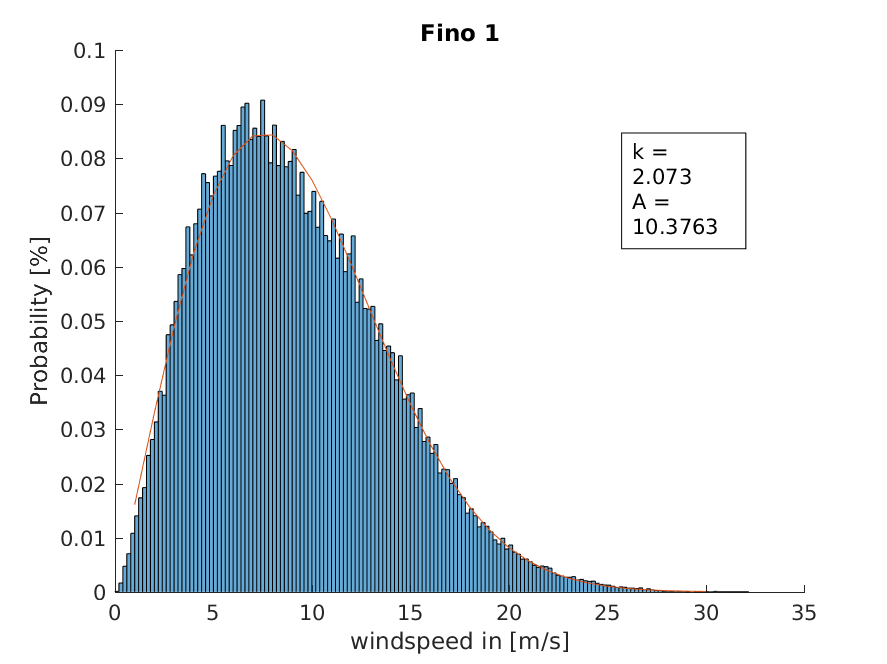
\includegraphics[width=1\linewidth]{../../figures/Hist_withfit_Fino1.png}
			\label{histo1}
		\end{minipage}
		\begin{minipage}[t]{0.49\linewidth}
		  \centering
		  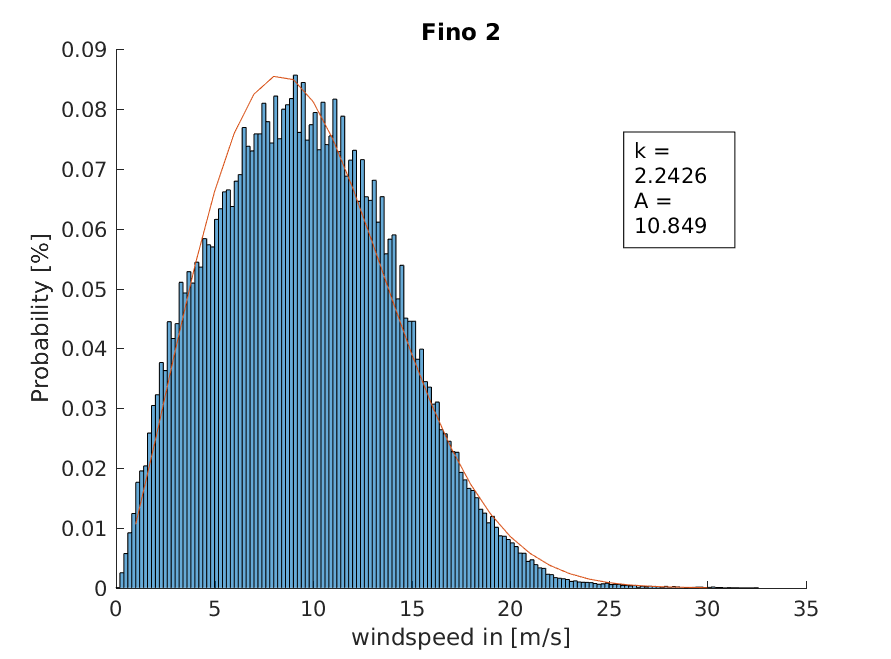
\includegraphics[width=1\linewidth]{../../figures/Hist_withfit_Fino2.png}
			\label{histo2}
		\end{minipage}
	\end{center}
\end{figure}
\end{frame}

\begin{frame}
\begin{figure}[htbp]
	\begin{center}
		\begin{minipage}[t]{0.45\linewidth}
			\centering
			Fino 1
			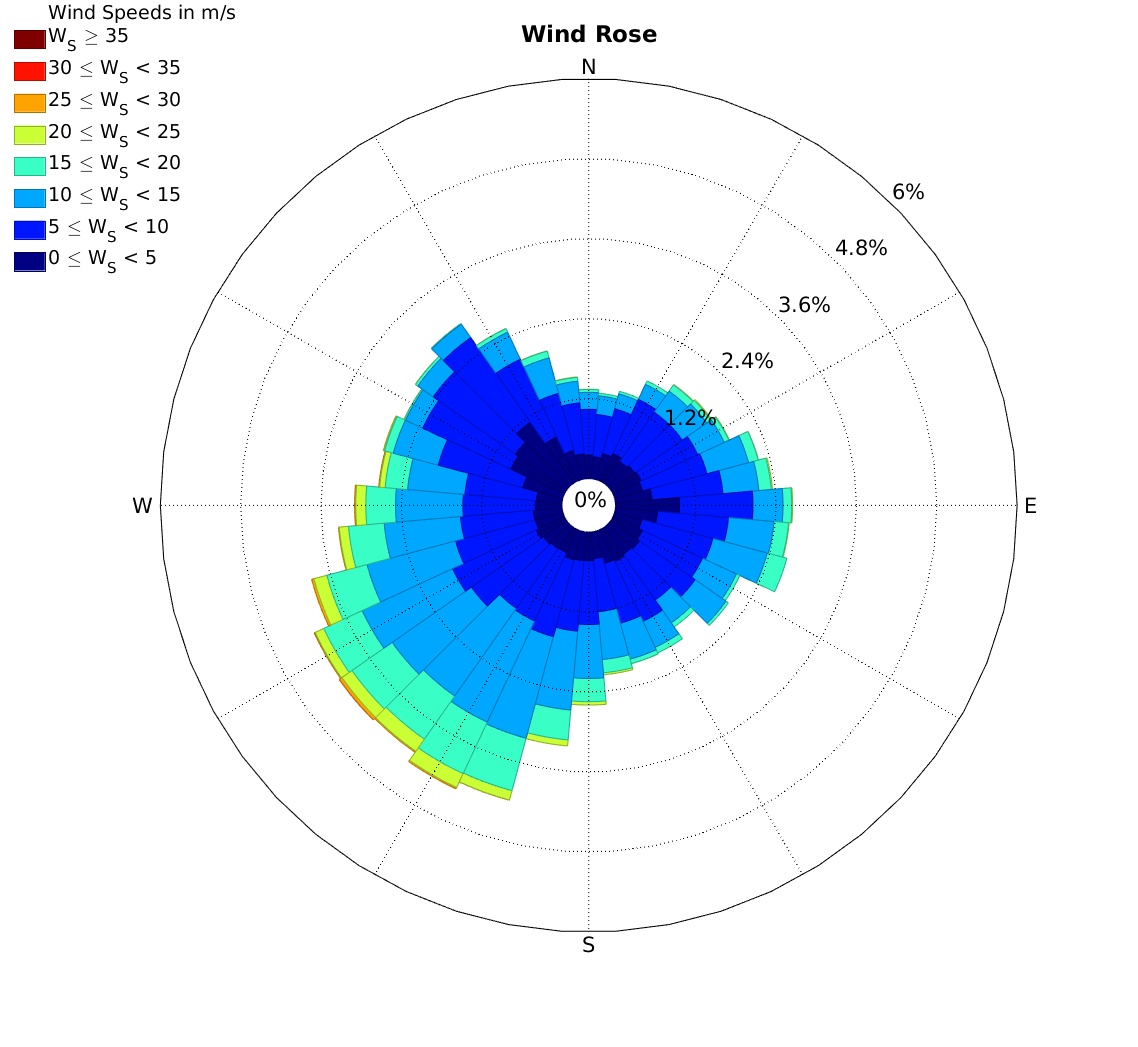
\includegraphics[width=\linewidth]{../../figures/WindRose_Fino1.png}
			
			
		\end{minipage}
		\begin{minipage}[t]{0.45\linewidth}
			\centering
			Fino 2
			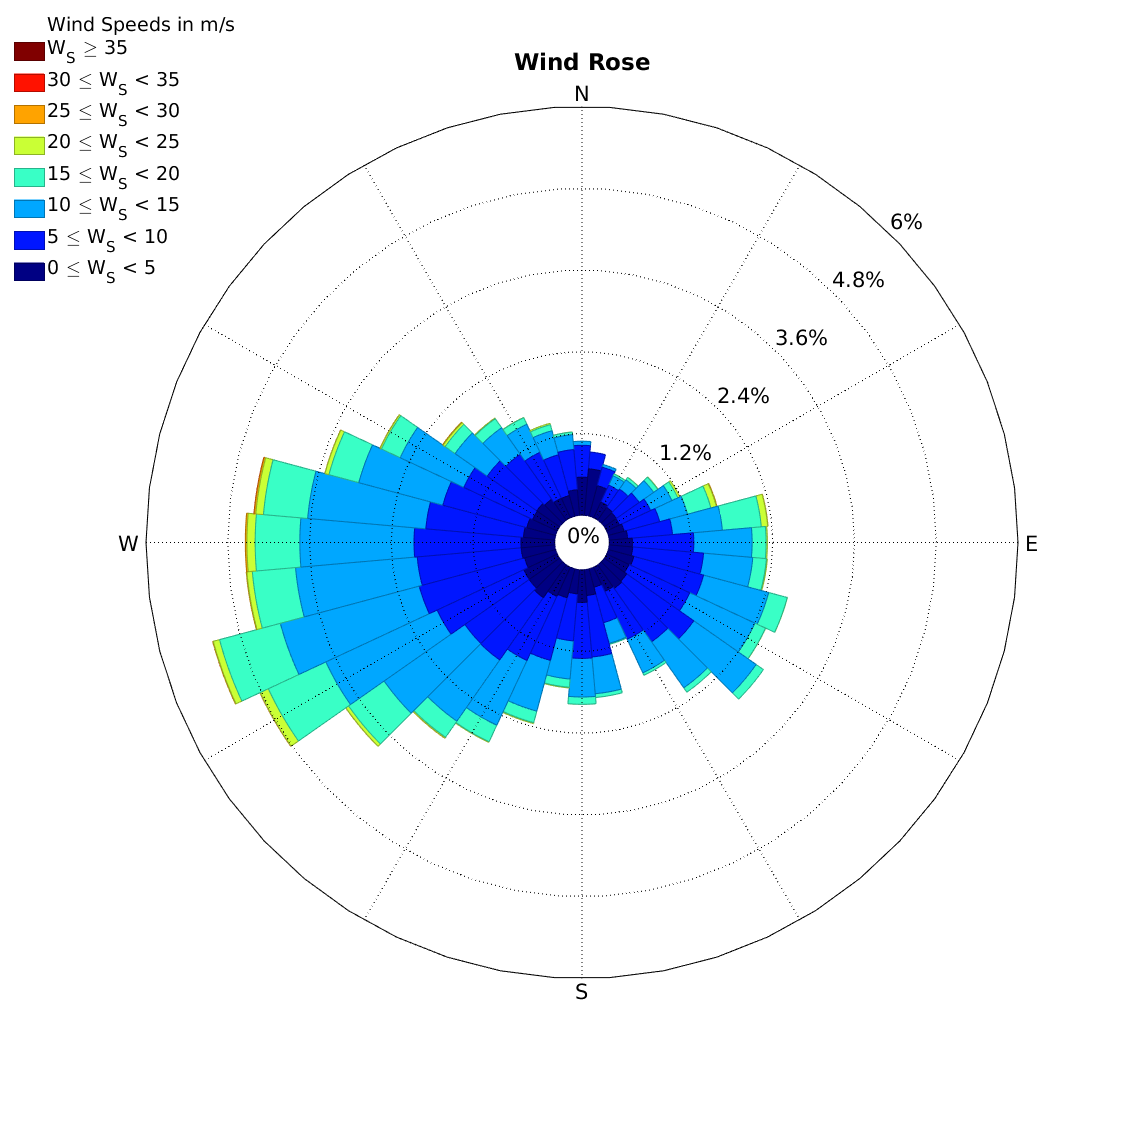
\includegraphics[width=\linewidth]{../../figures/WindRose_Fino2.png}

		\end{minipage}
	\end{center}
\end{figure}
\begin{tabular}{c| c| c}
			5y AEP 	& Fino 1 & Fino 2 \\ 
				\hline
			Vestas V90 1.8 MW & 39,3 GWh & 42,6 GWh \\
			\hline
			Enercon E82 3 MW& 46,4 GWh & 50,4 GWh \\
			\end{tabular}
\end{frame}


\section{Vertical wind speed profile}

\begin{frame}[fragile]
\frametitle{Non-linear regression of vertical profile}
\vspace{40 pt}
\begin{lstlisting}
logProfileModel = @(b,z) b(1)/0.4 *(log(z/b(2)));
logProfileCoeffs = nlinfit([33,40,50,60,70,80,90,100],avgPerHeight,logProfileModel,[0.2,10^-6],opts);
[x,y]=fplot(@(z) logProfileCoeffs(1)/0.4 *(log(z/logProfileCoeffs(2))),[0 100])

empPowerModel = @(c,x) avgPerHeight(8)*((x/90).^c(1));
empPowerCoeff = real(nlinfit([33,40,50,60,70,80,90,100],avgPerHeight,empPowerModel,[0.11],opts));
[x,y]=fplot(@(z) avgPerHeight(8)*(z/90)^(empPowerCoeff),[0 100]);
\end{lstlisting}
\end{frame}

\begin{frame}[fragile]
\frametitle{Vertical profile}
\begin{figure}[H]
\centering
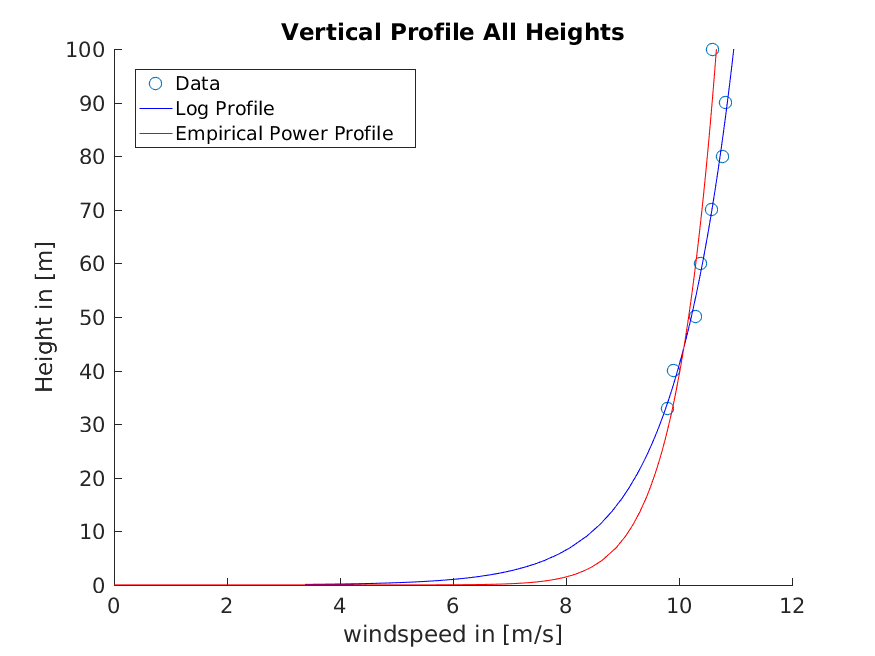
\includegraphics[width=0.8\linewidth]{../../figures/verticalProfileFits.png}
\label{fig:weatherpattern}
\end{figure}
\end{frame}


\begin{frame}[fragile]
\frametitle{Seasonal analysis of vertical profile}
\begin{figure}[htbp]
	\begin{center}
		\begin{minipage}[t]{0.49\linewidth}
			\centering
  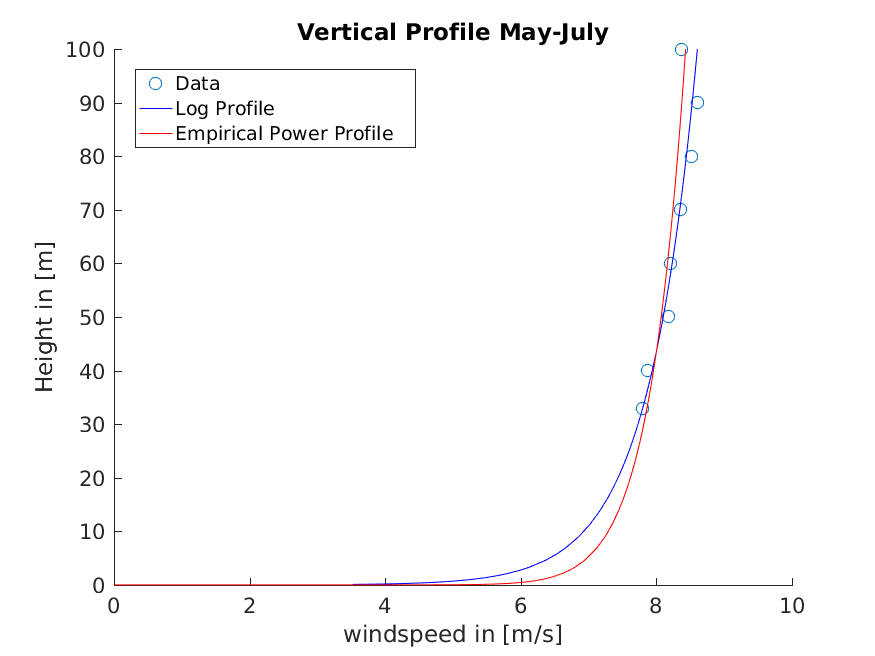
\includegraphics[width=1\linewidth]{../../figures/verticalProfileFitsSommer.png}
			\label{histo1}
		\end{minipage}
		\begin{minipage}[t]{0.49\linewidth}
		  \centering
  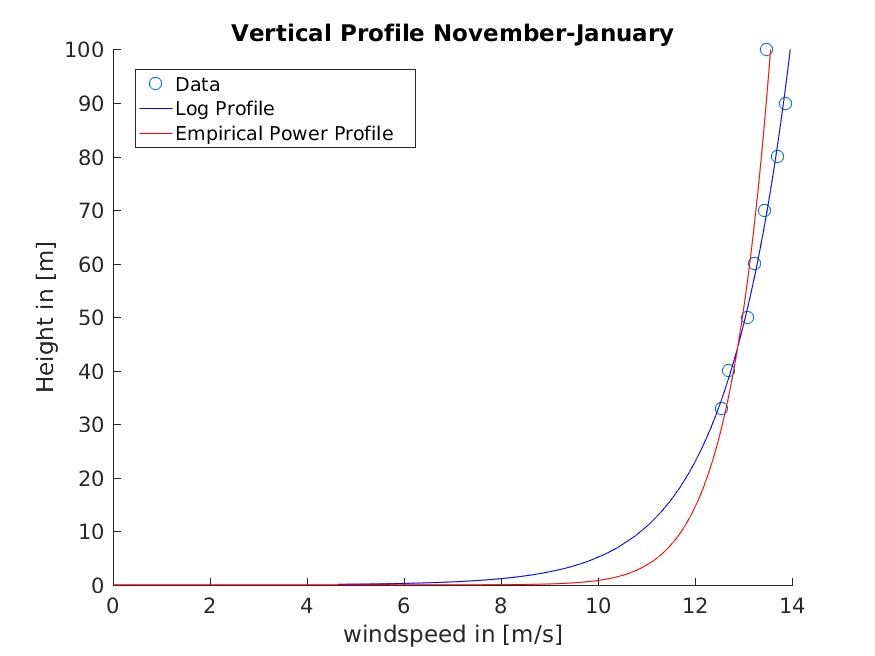
\includegraphics[width=1\linewidth]{../../figures/verticalProfileFitsWinter.png}
			\label{histo2}
		\end{minipage}
	\end{center}
\end{figure}
\end{frame}

\begin{frame}[fragile]
\frametitle{Comparison of regression models}
\begin{figure}[H]
\centering
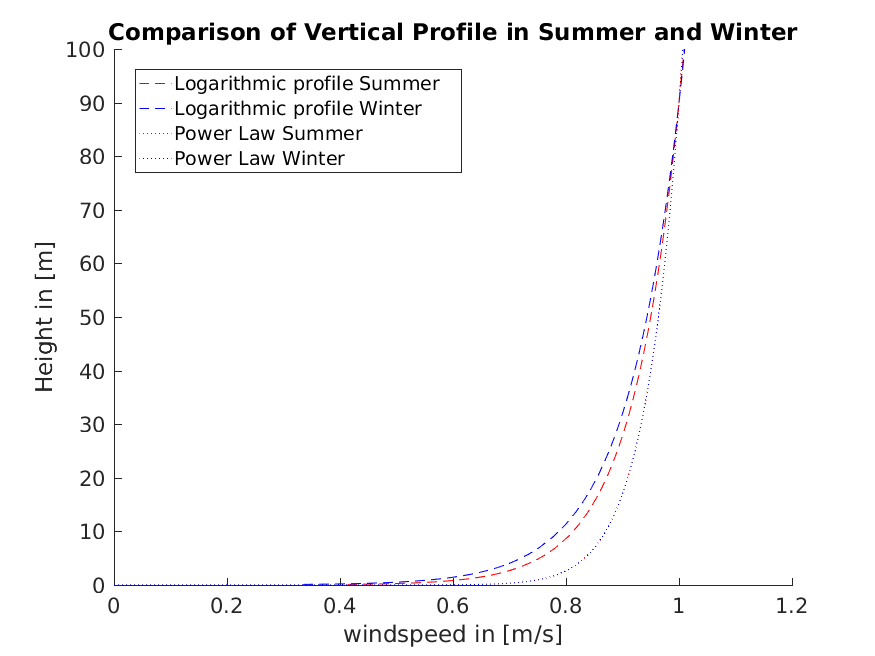
\includegraphics[width=0.8\linewidth]{../../figures/verticalProfilesComparison.png}
\label{fig:weatherpattern}
\end{figure}
\end{frame}

\begin{frame}[fragile]
\vspace{100 pt}
\Huge
\begin{center}
Thanks!
\end{center}
\end{frame}
%%%%%%%%%%%% End of content %%%%%%%%%%%%


\end{document}